% ============================================================================
% 4-MINUTE TALK — LaTeX (beamer) source, editable on Overleaf.
% Mirrors slides_4min.pptx one-for-one (same 7 slides, same numbers, same
% speaker notes). Compile with pdfLaTeX. Figures: fig1_arch.pdf (the report's
% Figure 1), eda_target.png, eda_temporal.png.
%
% Speaker notes are \note{...}; to print them, compile a second copy with
% \setbeameroption{show notes on second screen} or {show only notes}.
% ============================================================================
\documentclass[aspectratio=169,10pt]{beamer}

\usetheme{default}
\usecolortheme{default}
\setbeamertemplate{navigation symbols}{}
\setbeamertemplate{itemize items}[circle]

\usepackage[T1]{fontenc}
\usepackage[utf8]{inputenc}
\usepackage{helvet}
\renewcommand{\familydefault}{\sfdefault}
\usepackage{graphicx}
\usepackage{booktabs}
\usepackage{tikz}
\usepackage{xcolor}

% ---- Palette (matches the poster / report figures) -------------------------
\definecolor{navy}{RGB}{15,42,74}
\definecolor{ink}{RGB}{28,30,33}
\definecolor{mut}{RGB}{90,100,114}
\definecolor{ice}{RGB}{202,220,252}
\definecolor{barblue}{RGB}{43,108,176}
\definecolor{pale}{RGB}{168,189,212}
\definecolor{lt}{RGB}{244,247,251}
\definecolor{gold}{RGB}{138,109,26}

\setbeamercolor{normal text}{fg=ink}
\setbeamercolor{frametitle}{fg=navy}
\setbeamercolor{itemize item}{fg=navy}
\setbeamercolor{itemize subitem}{fg=navy}
\setbeamerfont{frametitle}{series=\bfseries, size=\Large}
\setbeamertemplate{frametitle}{%
  \vspace{4mm}\hspace{2mm}\insertframetitle\par\vspace{-1mm}}

% Dark title/closing frames
\newcommand{\darkframe}[1]{%
  \begingroup
  \setbeamercolor{background canvas}{bg=navy}
  #1
  \endgroup}

% Callout box
\newcommand{\callout}[2]{%
  \begin{tikzpicture}
    \node[fill=lt, draw=pale, line width=0.4pt, rounded corners=2pt,
          inner sep=3mm, text width=\dimexpr\linewidth-8mm] {%
      {\color{navy}\textbf{#1}}\\[1mm]{\small #2}};
  \end{tikzpicture}}

% Horizontal count bar: #1 label, #2 color, #3 fraction, #4 value
\newcommand{\countbar}[4]{%
  \noindent\makebox[16mm][l]{\scriptsize #1}%
  \begin{tikzpicture}[baseline=-0.9mm]
    \fill[lt] (0,0) rectangle (34mm,3mm);
    \fill[#2] (0,0) rectangle (#3*34mm,3mm);
  \end{tikzpicture}%
  \ \makebox[12mm][l]{\scriptsize #4}\par\vspace{1.4mm}}

\begin{document}

% ---------------------------------------------------------------- 1 TITLE --
{\setbeamercolor{background canvas}{bg=navy}
\begin{frame}[plain]
  \vspace{8mm}
  {\color{white}\Huge\bfseries AI Agents for\\[2mm] Kaggle Competitions\par}
  \vspace{6mm}
  {\color{ice}\large An end-to-end LLM agent, benchmarked against two frozen
   yardsticks on 20 Kaggle competitions\par}
  \vfill
  {\color{pale}\small Wei-Hao Huang \quad$\cdot$\quad Academia Sinica ISS
   Summer Internship 2026 \quad$\cdot$\quad Report v6 (2026-08-18)\par}
  \vspace{3mm}
  \note{Four minutes: what I built, how it works, what it scored, what
    surprised me, and what I would tell the next person. (10s)}
\end{frame}}

% ----------------------------------------------------------- 2 MOTIVATION --
\begin{frame}{Motivation --- why these tasks, why an agent}
  \begin{columns}[t]
    \begin{column}{0.48\textwidth}
      {\color{navy}\bfseries The challenge}
      \begin{itemize}\small
        \item Kaggle demands the full expert loop --- validation design,
          features, model selection, ensembling.
        \item Top entries differ at the 4th--5th decimal of the metric;
          intuition cannot rank them.
        \item Local cross-validation misleads: one competition scored
          6.71 out-of-fold yet 49.41 on the real leaderboard.
        \item EDA and diagnostic visualization are essential but repetitive
          for every new dataset.
      \end{itemize}
    \end{column}
    \begin{column}{0.48\textwidth}
      {\color{navy}\bfseries Why an AI agent fits}
      \begin{itemize}\small
        \item Tireless systematic search: 22--80 candidate configurations per
          competition, all logged.
        \item Holds one disciplined protocol across 20 competitions ---
          humans drift, agents don't.
        \item Emits EDA figures and per-competition reports automatically;
          every claim traces to an artifact.
      \end{itemize}
      \vspace{3mm}
      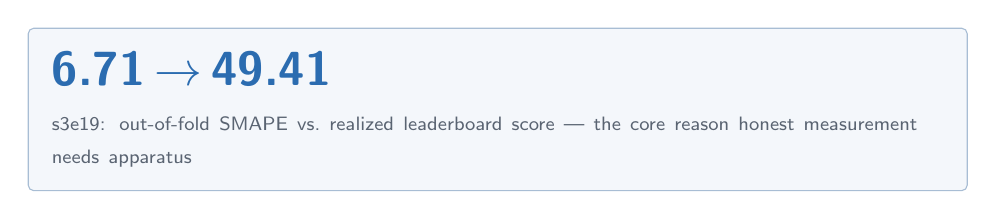
\begin{tikzpicture}
        \node[fill=lt, draw=pale, line width=0.4pt, rounded corners=2pt,
              inner sep=3mm, text width=\dimexpr\linewidth-8mm] {%
          {\color{barblue}\bfseries\LARGE 6.71 $\to$ 49.41}\\[1.5mm]
          {\color{mut}\scriptsize s3e19: out-of-fold SMAPE vs.\ realized
           leaderboard score --- the core reason honest measurement needs
           apparatus}};
      \end{tikzpicture}
    \end{column}
  \end{columns}
  \note{Kaggle is the full expert loop, and the margins are at the fourth
    decimal. The obvious compass --- your own cross-validation --- can be off
    by an order of magnitude: 6.71 out-of-fold became 49.41 on the real
    leaderboard. An agent fits because it is tireless, holds one protocol
    across 20 competitions, and documents everything it does. (35s)}
\end{frame}

% ------------------------------------------------------------- 3 WORKFLOW --
\begin{frame}{Workflow --- an LLM reasons at every stage}
  \begin{columns}[c]
    \begin{column}{0.46\textwidth}
      \centering
      
\includegraphics[width=\linewidth]{fig1_arch.pdf}\\[1mm]
      {\color{mut}\scriptsize\itshape Pipeline: dossier $\to$ EDA $\to$
       features $\to$ modeling $\to$ evaluation $\to$ submission $\to$ real
       leaderboard.}
    \end{column}
    \begin{column}{0.5\textwidth}
      \begin{itemize}\small
        \item LLM decides at every stage; Auto-ML tools (LightGBM / XGBoost /
          CatBoost / Optuna) do the heavy lifting via the shell.
        \item Experience library: cross-competition priors, every entry
          evidence-backed, written back after each run.
        \item Tree search over candidate configurations is the optimisation
          loop --- ensembles are first-class nodes with OOF caching.
        \item Stage-0.5 dossier (injection layer): classifies the task and
          injects external data upstream, before any modeling.
      \end{itemize}
    \end{column}
  \end{columns}
  \note{The workflow: data ingestion, a problem dossier, EDA, features,
    modeling, evaluation, submission. The LLM reasons at every stage and
    drives Auto-ML tools through the shell. Two things make it more than a
    script: an evidence-backed experience library shared across competitions,
    and a tree search where ensembles are first-class nodes. (40s)}
\end{frame}

% ------------------------------------------------ 4 RESULTS: LEADERBOARDS --
\begin{frame}{Results --- my-agent on real leaderboards}
  \begin{columns}[t]
    \begin{column}{0.47\textwidth}
      {\color{navy}\bfseries\small Best private score across the 16 scored
       competitions}\\[3mm]
      \countbar{my-agent}{barblue}{0.625}{10 / 16}
      \countbar{NVIDIA}{pale}{0.3125}{5 / 16}
      \countbar{AIDE}{pale}{0.0625}{1 / 16}
      \vspace{2mm}
      {\color{mut}\scriptsize 16 of 20 lanes are scored on the real
       leaderboard, adjudicated by a paired test on Kaggle's public/private
       split: my-agent stands 15 W / 5 L (75\% excl.\ ties). On s3e19 the
       dossier layer's external-data injection turns the canonical failure
       (SMAPE 50.455 without the layer) into a numerical first among the three
       agents (48.243), and all 6 of 6 controlled arms beat their matched
       baselines.}
    \end{column}
    \begin{column}{0.49\textwidth}
      {\color{navy}\bfseries\small Beyond tabular --- my-agent beats both
       yardsticks on all three}\\[2mm]
      {\scriptsize\setlength{\tabcolsep}{1.1mm}%
      \begin{tabular}{@{}llrrr@{}}
        \toprule
        \textbf{Competition} & \textbf{Metric} & \textbf{my-agent} &
          \textbf{NVIDIA} & \textbf{AIDE}\\
        \midrule
        us-patent & Pearson $r$ $\uparrow$ &
          {\color{barblue}\bfseries 0.86658} & 0.86160 & 0.65821\\
        ventilator & MAE $\downarrow$ &
          {\color{barblue}\bfseries 0.16525} & 0.40093 & 0.34591\\
        SIIM-ISIC & AUC $\uparrow$ &
          {\color{barblue}\bfseries 0.93529} & 0.89822 & 0.88579\\
        \bottomrule
      \end{tabular}\par}
      \vspace{4mm}
      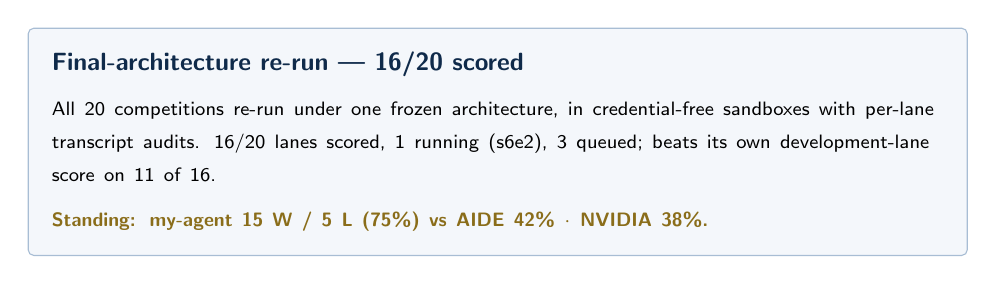
\begin{tikzpicture}
        \node[fill=lt, draw=pale, line width=0.4pt, rounded corners=2pt,
              inner sep=3mm, text width=\dimexpr\linewidth-8mm] {%
          {\color{navy}\bfseries\small Final-architecture re-run --- 16/20
           scored}\\[1.5mm]
          {\scriptsize All 20 competitions re-run under one frozen
           architecture, in credential-free sandboxes with per-lane transcript
           audits. 16/20 lanes scored, 1 running (s6e2), 3 queued; beats its
           own development-lane score on 11 of 16.}\\[1.5mm]
          {\color{gold}\scriptsize\bfseries Standing: my-agent 15 W / 5 L
           (75\%) vs AIDE 42\% $\cdot$ NVIDIA 38\%.}};
      \end{tikzpicture}
    \end{column}
  \end{columns}
  \note{Sixteen of twenty lanes are scored on the real leaderboard under the
    frozen architecture: fifteen wins, five losses --- seventy-five percent ---
    against forty-two percent for AIDE and thirty-eight for NVIDIA, with the
    best private score on ten of sixteen. The injection layer turns our worst
    competition into a numerical first among the three agents, six of six
    controlled arms beat their baselines, and on the three harder competitions
    outside tabular data my agent takes the best score on all three. (45s)}
\end{frame}

% ----------------------------------------------- 5 RESULTS: VISUALIZATION --
\begin{frame}{Results --- the agent's visualization output}
  \centering
  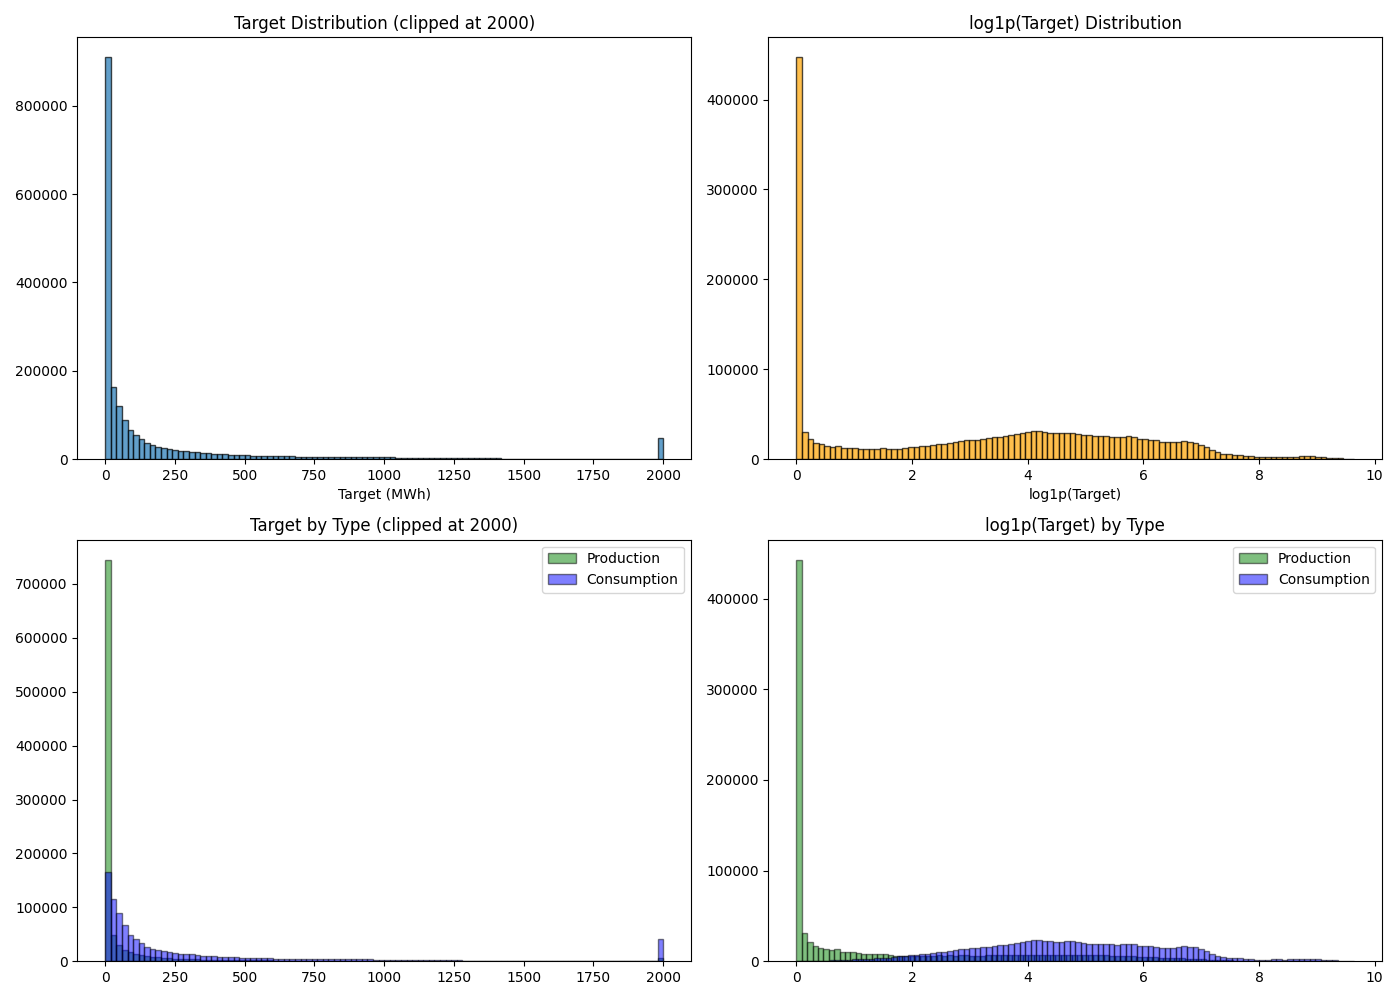
\includegraphics[height=0.52\textheight]{eda_target.png}\hfill
  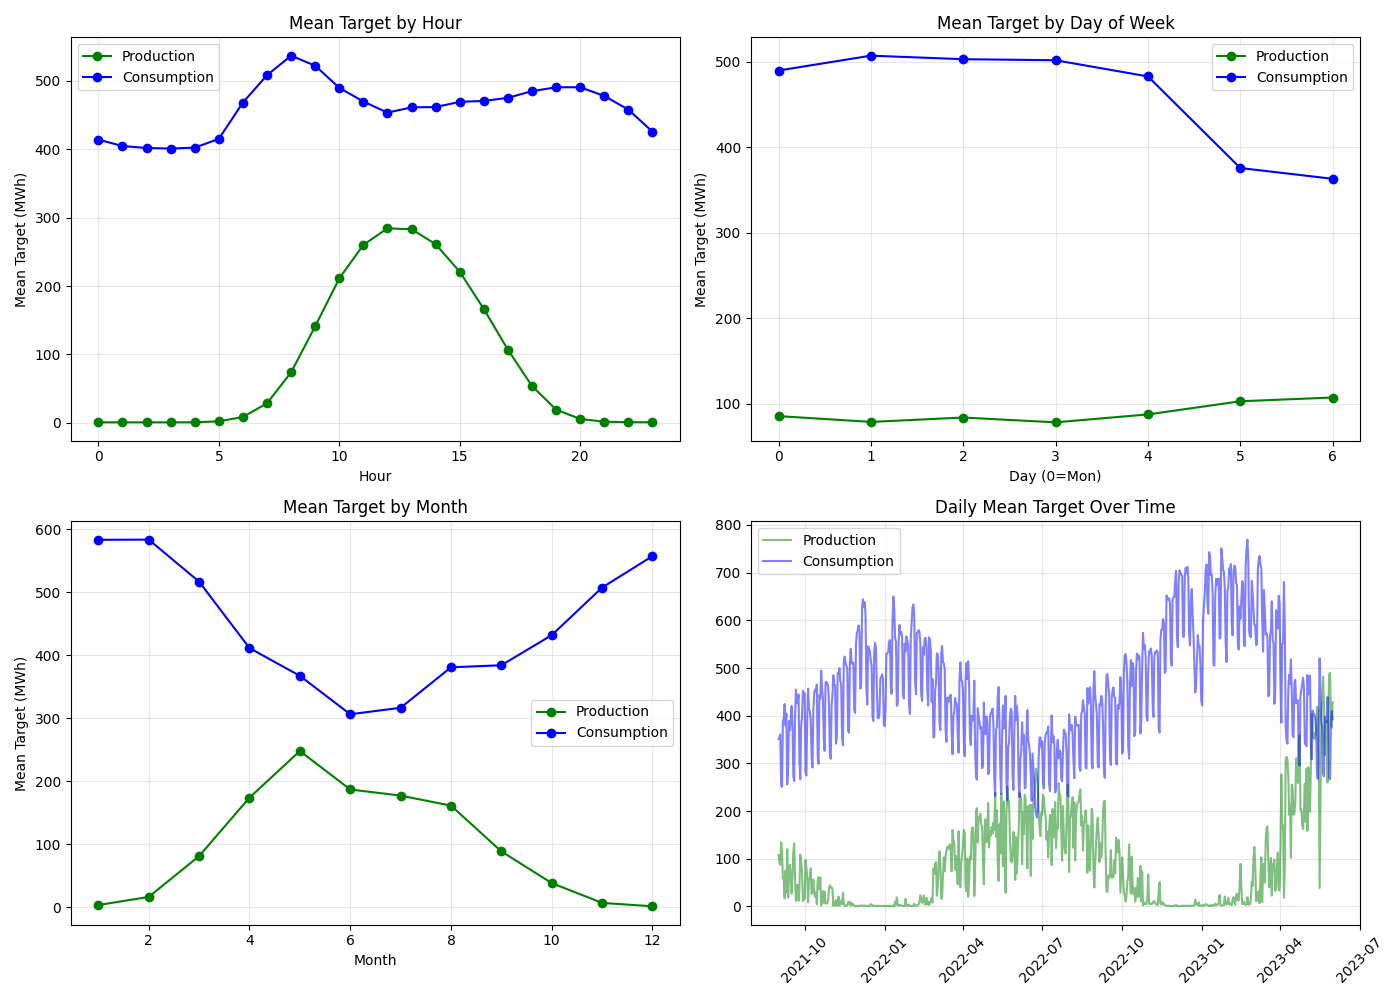
\includegraphics[height=0.52\textheight]{eda_temporal.png}\\[2mm]
  {\color{mut}\scriptsize Agent-generated EDA, produced automatically before
   modeling (energy-prosumer example): target distributions by segment (left)
   and temporal consumption/production patterns (right). The same pipeline
   emits 22 per-competition ML-spec reports and its own architecture
   flowcharts.}
  \note{The visualization half: before any modeling, the agent draws its own
    diagnostics --- distributions, temporal patterns, drift checks --- and it
    writes 22 per-competition specification reports. Every figure you see in
    the report and the poster was produced by the pipeline itself. (25s)}
\end{frame}

% --------------------------------------------------- 6 EXPECTED VS ACTUAL --
\begin{frame}{What I expected vs.\ what I experienced}
  \small
  \begin{columns}[t]
    \begin{column}{0.40\textwidth}
      {\color{mut}\bfseries Expected}
    \end{column}
    \begin{column}{0.56\textwidth}
      {\color{navy}\bfseries Experienced}
    \end{column}
  \end{columns}
  \vspace{2mm}
  \begin{columns}[t]
    \begin{column}{0.40\textwidth}\scriptsize\itshape\color{mut}
      The agent would quickly beat most humans.\\[5.5mm]
      One run and one score decide a winner.\\[5.5mm]
      The agent follows the rules by default.\\[5.5mm]
      Fairness is mostly a mindset.
    \end{column}
    \begin{column}{0.56\textwidth}\scriptsize
      Scored frozen-architecture runs stand 15 W / 5 L (75\%) with the best
      private score on 10 of 16 lanes; wins concentrate where no mature public
      solutions exist.\\[2.5mm]
      Score noise + run variance leave close duels undecidable on a single
      score; a paired error model became mandatory.\\[2.5mm]
      A transcript audit caught a lane reading its own competition's recorded
      findings --- the clean re-run's local validation scored worse,
      consistent with a real contamination advantage.\\[2.5mm]
      It is infrastructure: isolated data roots, credential-free sandboxes,
      per-lane audits --- expensive, but without them numbers aren't
      comparable.
    \end{column}
  \end{columns}
  \note{What surprised me. I expected the agent to beat most humans quickly
    --- it wins fifteen of twenty scored head-to-heads, and its edge
    concentrates where no public solutions exist. I expected one score to
    decide a winner --- close duels are undecidable without a paired error
    model. And I expected rule-following by default --- the transcript audit
    proved otherwise once, and proved itself once by a false positive. (40s)}
\end{frame}

% ------------------------------------------------------------- 7 DISCUSSION --
{\setbeamercolor{background canvas}{bg=navy}
\begin{frame}[plain]
  \vspace{4mm}
  {\color{white}\Large\bfseries Advice --- if you use an AI agent for this\par}
  \vspace{6mm}
  {\color{ice}\small
  \begin{itemize}\setlength{\itemsep}{2.5mm}
    \item \textbf{State the error model with every claim.} Without an error
      scale a ranking is noise: close duels are undecidable, and the winner
      flips when the evaluation set changes.
    \item \textbf{Never trust local CV for between-agent claims} --- score on
      the real leaderboard.
    \item \textbf{Freeze your yardsticks.} Improving a baseline mid-study turns
      the benchmark into an optimisation of the baseline.
    \item \textbf{Isolate mechanically, then audit the transcript} --- reading
      what the agent actually did catches the leaks you didn't anticipate, in
      both directions.
    \item \textbf{Put knowledge injection upstream}: at the blend stage it was
      worth ${\sim}10^{-5}$; moved into problem identification it lifted the
      canonical failure case from last to first.
  \end{itemize}\par}
  \vfill
  {\color{pale}\scriptsize Report v6 $\cdot$ Engineering Log $\cdot$ Case
   Studies $\cdot$ 22 ML-spec reports \quad---\quad
   github.com/930731haohao-afk/kaggle-agent\par}
  \vspace{3mm}
  \note{If you do this yourself: state an error model with every claim, never
    trust local CV between agents, freeze your yardsticks, isolate
    mechanically and then read the transcript, and put knowledge injection
    upstream. Everything is in report v6 and the repository. Thank you. (25s)}
\end{frame}}

\end{document}
